\documentclass{article}
\usepackage{fontspec,tikz,graphicx}
\setmainfont{Times New Roman}
\usepackage[a3paper,margin=1cm]{geometry}
\pagestyle{empty}
\begin{document}
\noindent\resizebox{\textwidth}{!}{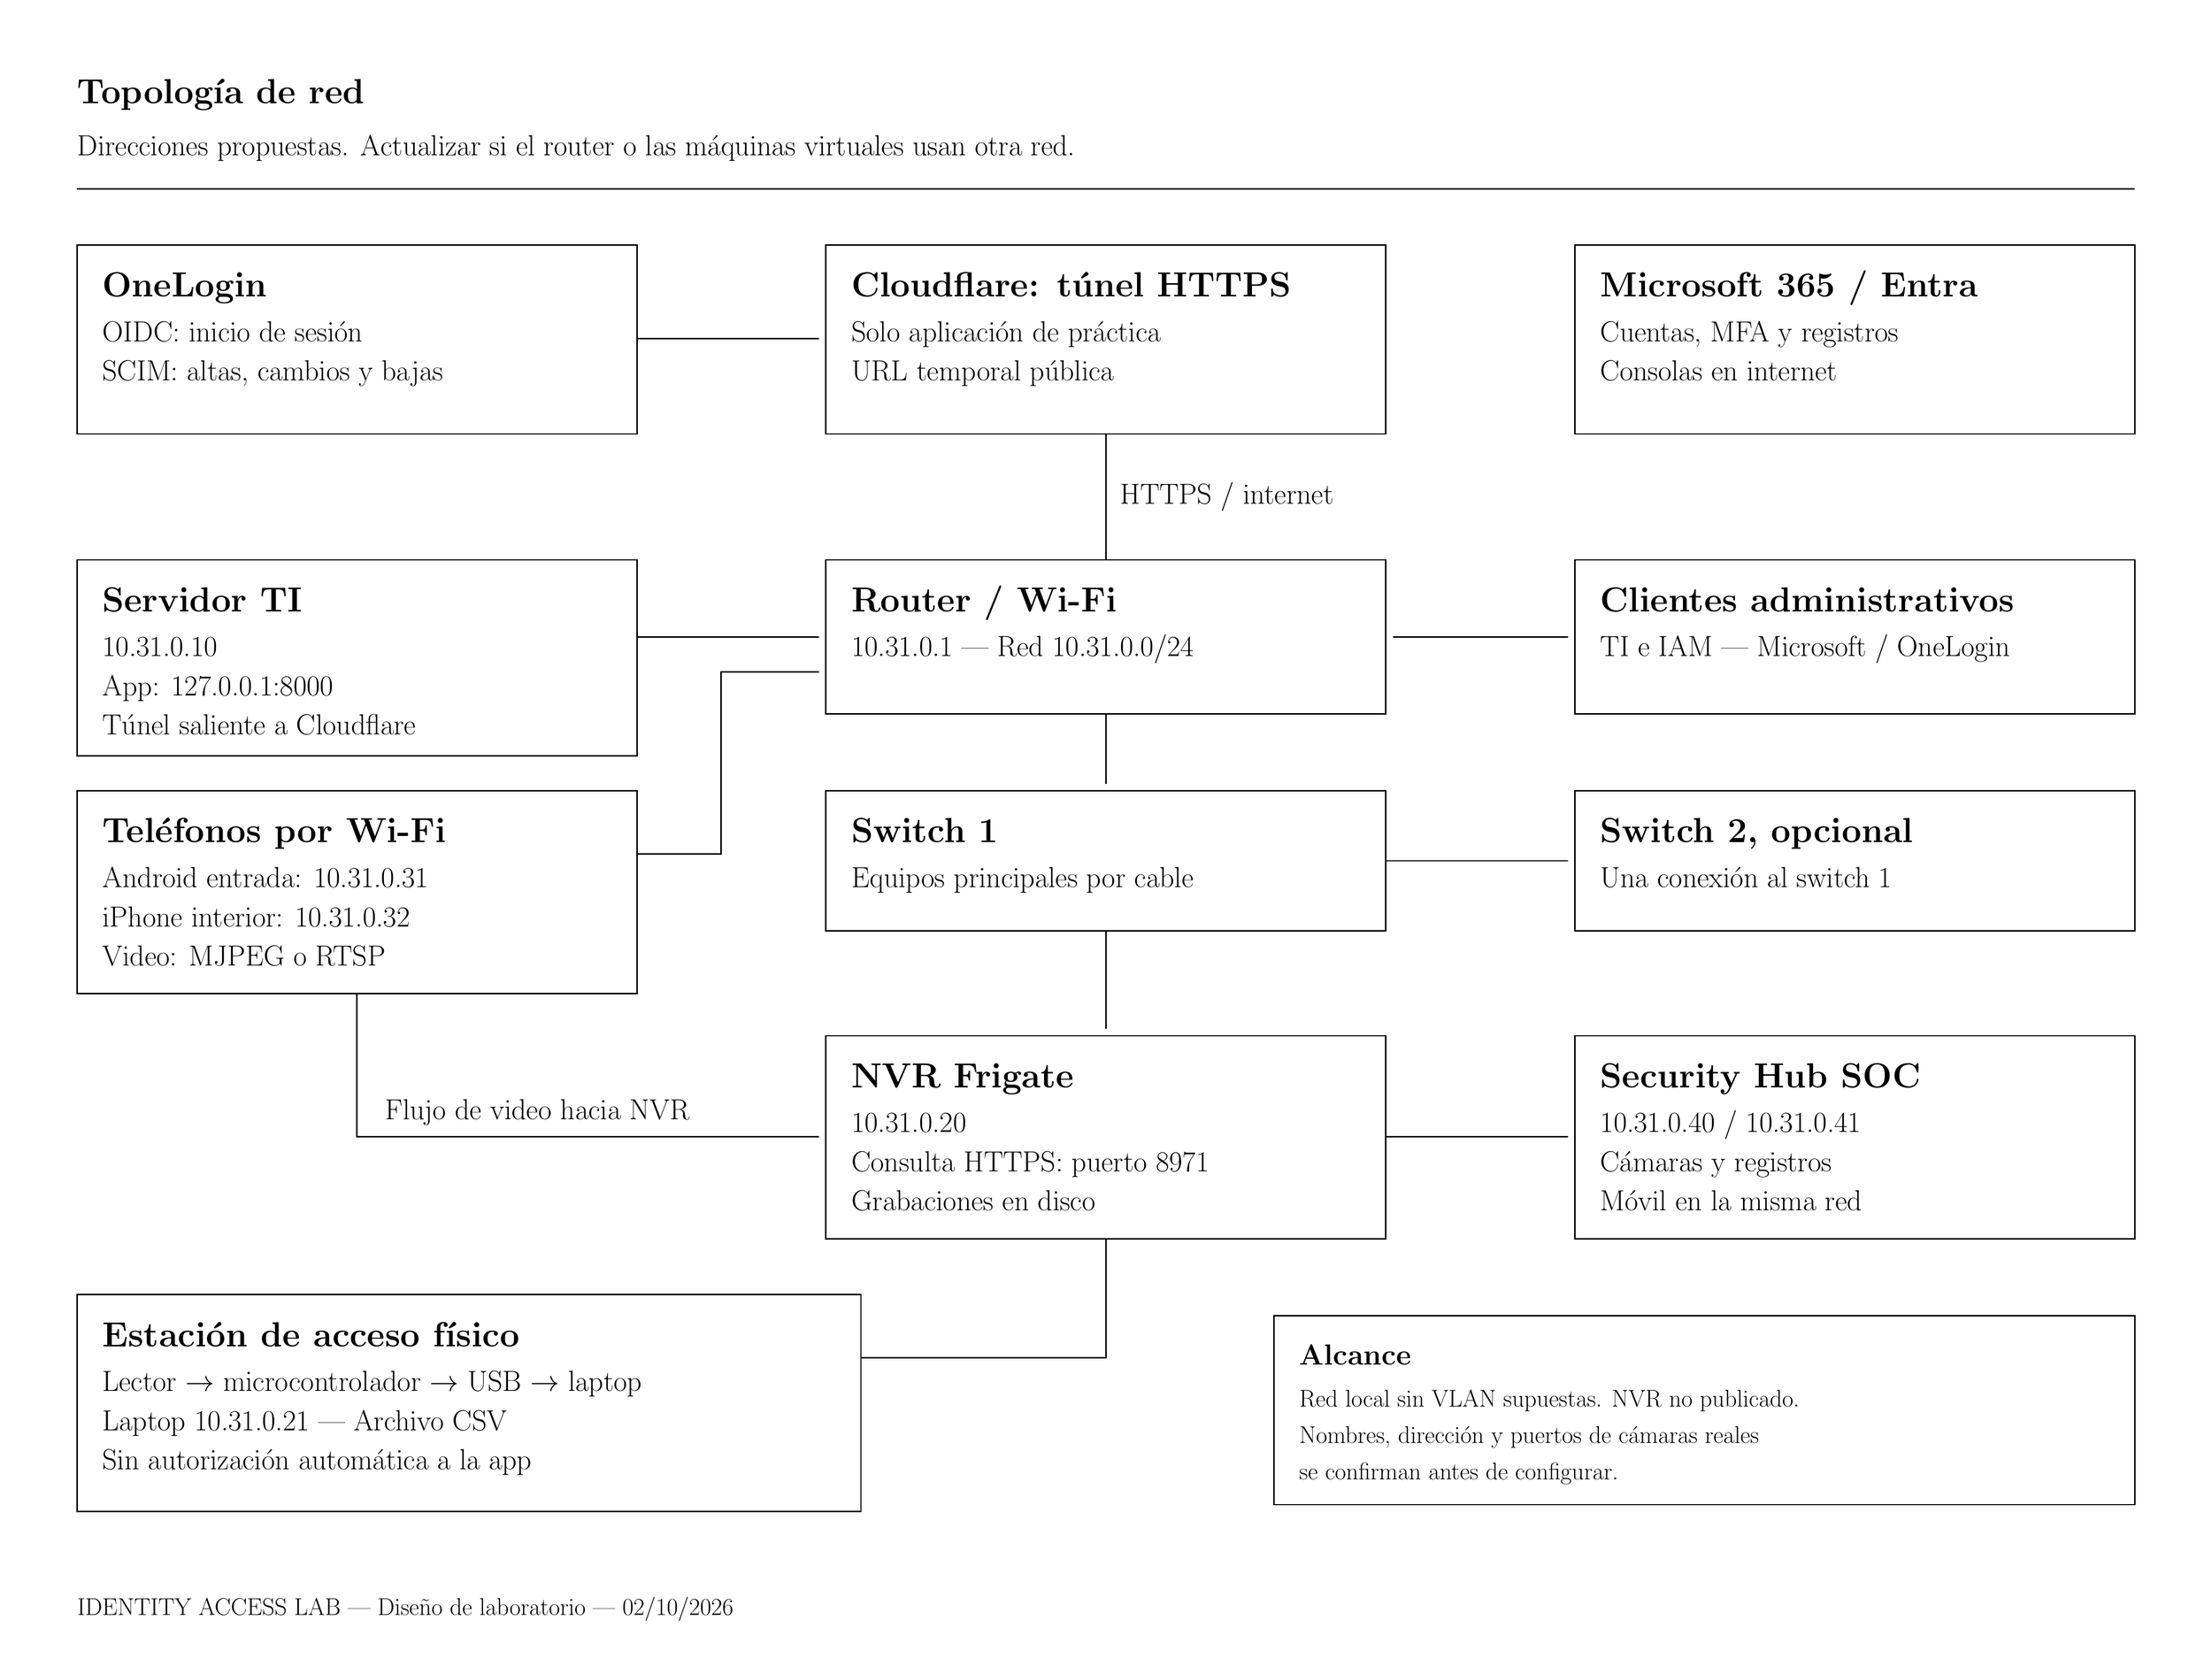
\begin{tikzpicture}[x=1pt,y=-1pt]
\path[use as bounding box] (0,0) rectangle (1560.0,1170.0);
\node[anchor=base west,inner sep=0pt,font=\fontsize{34.0}{40.8}\selectfont \bfseries ] at (45,64) {Topología de red};
\node[anchor=base west,inner sep=0pt,font=\fontsize{21.0}{25.2}\selectfont ] at (45,101) {Direcciones propuestas. Actualizar si el router o las máquinas virtuales usan otra red.};
\draw[line width=1pt] (45,125) -- (1515,125);
\draw[line width=1pt] (45.0,165.0) rectangle (445.0,300.0);
\node[anchor=base west,inner sep=0pt,font=\fontsize{23.0}{27.599999999999998}\selectfont \bfseries ] at (63,202) {OneLogin};
\node[anchor=base west,inner sep=0pt,font=\fontsize{21.0}{25.2}\selectfont ] at (63,234) {OIDC: inicio de sesión};
\node[anchor=base west,inner sep=0pt,font=\fontsize{21.0}{25.2}\selectfont ] at (63,262) {SCIM: altas, cambios y bajas};
\draw[line width=1pt] (580.0,165.0) rectangle (980.0,300.0);
\node[anchor=base west,inner sep=0pt,font=\fontsize{23.0}{27.599999999999998}\selectfont \bfseries ] at (598,202) {Cloudflare: túnel HTTPS};
\node[anchor=base west,inner sep=0pt,font=\fontsize{21.0}{25.2}\selectfont ] at (598,234) {Solo aplicación de práctica};
\node[anchor=base west,inner sep=0pt,font=\fontsize{21.0}{25.2}\selectfont ] at (598,262) {URL temporal pública};
\draw[line width=1pt] (1115.0,165.0) rectangle (1515.0,300.0);
\node[anchor=base west,inner sep=0pt,font=\fontsize{23.0}{27.599999999999998}\selectfont \bfseries ] at (1133,202) {Microsoft 365 / Entra};
\node[anchor=base west,inner sep=0pt,font=\fontsize{21.0}{25.2}\selectfont ] at (1133,234) {Cuentas, MFA y registros};
\node[anchor=base west,inner sep=0pt,font=\fontsize{21.0}{25.2}\selectfont ] at (1133,262) {Consolas en internet};
\draw[line width=1pt] (445,232) -- (575,232);
\draw[line width=1pt] (780,300) -- (780,390);
\node[anchor=base west,inner sep=0pt,font=\fontsize{20.0}{24.0}\selectfont ] at (790,350) {HTTPS / internet};
\draw[line width=1pt] (580.0,390.0) rectangle (980.0,500.0);
\node[anchor=base west,inner sep=0pt,font=\fontsize{23.0}{27.599999999999998}\selectfont \bfseries ] at (598,427) {Router / Wi-Fi};
\node[anchor=base west,inner sep=0pt,font=\fontsize{21.0}{25.2}\selectfont ] at (598,459) {10.31.0.1 | Red 10.31.0.0/24};
\draw[line width=1pt] (45.0,390.0) rectangle (445.0,530.0);
\node[anchor=base west,inner sep=0pt,font=\fontsize{23.0}{27.599999999999998}\selectfont \bfseries ] at (63,427) {Servidor TI};
\node[anchor=base west,inner sep=0pt,font=\fontsize{21.0}{25.2}\selectfont ] at (63,459) {10.31.0.10};
\node[anchor=base west,inner sep=0pt,font=\fontsize{21.0}{25.2}\selectfont ] at (63,487) {App: 127.0.0.1:8000};
\node[anchor=base west,inner sep=0pt,font=\fontsize{21.0}{25.2}\selectfont ] at (63,515) {Túnel saliente a Cloudflare};
\draw[line width=1pt] (445,445) -- (575,445);
\draw[line width=1pt] (1115.0,390.0) rectangle (1515.0,500.0);
\node[anchor=base west,inner sep=0pt,font=\fontsize{23.0}{27.599999999999998}\selectfont \bfseries ] at (1133,427) {Clientes administrativos};
\node[anchor=base west,inner sep=0pt,font=\fontsize{21.0}{25.2}\selectfont ] at (1133,459) {TI e IAM | Microsoft / OneLogin};
\draw[line width=1pt] (985,445) -- (1110,445);
\draw[line width=1pt] (580.0,555.0) rectangle (980.0,655.0);
\node[anchor=base west,inner sep=0pt,font=\fontsize{23.0}{27.599999999999998}\selectfont \bfseries ] at (598,592) {Switch 1};
\node[anchor=base west,inner sep=0pt,font=\fontsize{21.0}{25.2}\selectfont ] at (598,624) {Equipos principales por cable};
\draw[line width=1pt] (780,500) -- (780,550);
\draw[line width=1pt] (45.0,555.0) rectangle (445.0,700.0);
\node[anchor=base west,inner sep=0pt,font=\fontsize{23.0}{27.599999999999998}\selectfont \bfseries ] at (63,592) {Teléfonos por Wi-Fi};
\node[anchor=base west,inner sep=0pt,font=\fontsize{21.0}{25.2}\selectfont ] at (63,624) {Android entrada: 10.31.0.31};
\node[anchor=base west,inner sep=0pt,font=\fontsize{21.0}{25.2}\selectfont ] at (63,652) {iPhone interior: 10.31.0.32};
\node[anchor=base west,inner sep=0pt,font=\fontsize{21.0}{25.2}\selectfont ] at (63,680) {Video: MJPEG o RTSP};
\draw[line width=1pt] (445,600) -- (505,600) -- (505,470) -- (575,470);
\draw[line width=1pt] (1115.0,555.0) rectangle (1515.0,655.0);
\node[anchor=base west,inner sep=0pt,font=\fontsize{23.0}{27.599999999999998}\selectfont \bfseries ] at (1133,592) {Switch 2, opcional};
\node[anchor=base west,inner sep=0pt,font=\fontsize{21.0}{25.2}\selectfont ] at (1133,624) {Una conexión al switch 1};
\draw[line width=1pt] (980,605) -- (1110,605);
\draw[line width=1pt] (580.0,730.0) rectangle (980.0,875.0);
\node[anchor=base west,inner sep=0pt,font=\fontsize{23.0}{27.599999999999998}\selectfont \bfseries ] at (598,767) {NVR Frigate};
\node[anchor=base west,inner sep=0pt,font=\fontsize{21.0}{25.2}\selectfont ] at (598,799) {10.31.0.20};
\node[anchor=base west,inner sep=0pt,font=\fontsize{21.0}{25.2}\selectfont ] at (598,827) {Consulta HTTPS: puerto 8971};
\node[anchor=base west,inner sep=0pt,font=\fontsize{21.0}{25.2}\selectfont ] at (598,855) {Grabaciones en disco};
\draw[line width=1pt] (780,655) -- (780,725);
\draw[line width=1pt] (245,700) -- (245,802) -- (575,802);
\node[anchor=base west,inner sep=0pt,font=\fontsize{20.0}{24.0}\selectfont ] at (265,790) {Flujo de video hacia NVR};
\draw[line width=1pt] (1115.0,730.0) rectangle (1515.0,875.0);
\node[anchor=base west,inner sep=0pt,font=\fontsize{23.0}{27.599999999999998}\selectfont \bfseries ] at (1133,767) {Security Hub SOC};
\node[anchor=base west,inner sep=0pt,font=\fontsize{21.0}{25.2}\selectfont ] at (1133,799) {10.31.0.40 / 10.31.0.41};
\node[anchor=base west,inner sep=0pt,font=\fontsize{21.0}{25.2}\selectfont ] at (1133,827) {Cámaras y registros};
\node[anchor=base west,inner sep=0pt,font=\fontsize{21.0}{25.2}\selectfont ] at (1133,855) {Móvil en la misma red};
\draw[line width=1pt] (980,802) -- (1110,802);
\draw[line width=1pt] (45.0,915.0) rectangle (605.0,1070.0);
\node[anchor=base west,inner sep=0pt,font=\fontsize{23.0}{27.599999999999998}\selectfont \bfseries ] at (63,952) {Estación de acceso físico};
\node[anchor=base west,inner sep=0pt,font=\fontsize{21.0}{25.2}\selectfont ] at (63,984) {Lector \(\rightarrow\) microcontrolador \(\rightarrow\) USB \(\rightarrow\) laptop};
\node[anchor=base west,inner sep=0pt,font=\fontsize{21.0}{25.2}\selectfont ] at (63,1012) {Laptop 10.31.0.21 | Archivo CSV};
\node[anchor=base west,inner sep=0pt,font=\fontsize{21.0}{25.2}\selectfont ] at (63,1040) {Sin autorización automática a la app};
\draw[line width=1pt] (605,960) -- (780,960) -- (780,875);
\draw[line width=1pt] (900.0,930.0) rectangle (1515.0,1065.0);
\node[anchor=base west,inner sep=0pt,font=\fontsize{21.0}{25.2}\selectfont \bfseries ] at (918,965) {Alcance};
\node[anchor=base west,inner sep=0pt,font=\fontsize{19.0}{22.8}\selectfont ] at (918,995) {Red local sin VLAN supuestas. NVR no publicado.};
\node[anchor=base west,inner sep=0pt,font=\fontsize{19.0}{22.8}\selectfont ] at (918,1021) {Nombres, dirección y puertos de cámaras reales};
\node[anchor=base west,inner sep=0pt,font=\fontsize{19.0}{22.8}\selectfont ] at (918,1047) {se confirman antes de configurar.};
\node[anchor=base west,inner sep=0pt,font=\fontsize{18.0}{21.599999999999998}\selectfont ] at (45,1144) {IDENTITY ACCESS LAB | Diseño de laboratorio | 02/10/2026};
\end{tikzpicture}}
\end{document}
